
%% Template base para a elaboração do trabalho completo a ser enviado ao XIV Simpósio Brasileiro de Engenharia Física 

\documentclass[por]{Template_SBEF}

% Título do trabalho
\title{ESTIMATIVA DE PARÂMETROS PARA PROCESSOS CROMATOGRÁFICOS EM LEITO MÓVEL SIMULADO}

% Título curto
\shorttitle{ESTIMATIVA DE PARÂMETROS PARA PROCESSOS CROMATOGRÁFICOS}
      
% Autores
\author[1]{Pedro Pacheco Mendes Filho}
\author[2]{Claudir Oliveira}
\author[3]{Josecley Fialho Góes}

% Afiliações dos autores
\affil[1]{Instituto de Engenharia e Geociência, UFOPA, Santarém - Pará, Brasil}
\affil[2]{Instituto de Ciências da Educação, UFOPA, , Santarém - Pará, Brasil}
\affil[3]{Instituto de Engenharia e Geociência, UFOPA, Santarém - Pará, Brasil}

% Sobrenome do primeiro autor
\firstauthor{Pacheco, Pedro}

% correspondência principal
\email{domprechecopa@gmail.com}            
\newcommand{\vect}[1]{\mathbf{#1}}


% Iniciar documento
\begin{document}
\resumo{Em aplicações nas indústrias, a cromatografia em sistema de Leito Móvel Simulado (LMS) é utilizado na separação e purificação de misturas. Na modelagem matemática dos fenômenos envolvidos, a estimativa de parâmteros para as etapas de separação é um fator fundamental para conseguir grandes avanços no processo de transporte de massa. O objetivo deste trabalho consiste no uso da abordagem de problemas inversos para determinar parâmetros em um sistema de LMS, composto por oito colunas e quatro seções, usando a estimativa por \textit{Máxima Verossimilhança}  e \textit{Máximo a Posteriori} via algoritmo de Evolução Diferencial. Utilizou-se o modelo de Transporte Dispersivo a representação das colunas que compôem o LMS e na solução do problema direto considerou-se uma simulação de separação do 1,1’-bi-2-naftol, por ser um dos constituintes bastante procurado em processos quiral. A isoterma bi-Langmuir foi usada para descrever o equilíbrio entre as fases líquida e sólida na separação dos enantiômeros. Para a solução do problema inverso, a modelagem matemática de problema direto foi validada por meio de dados experimentais obtidos na literatura. O sistema de equações diferenciais resultante da modelagem das colunas do LMS é resolvido via método de Runge-Kutta de quarta ordem.}

%palavras-chave
\palabrasclave{Problemas Inversos, Estimativa de Parâmetros, Método Estocástico, Separação de Substância, Transporte de Massa.}

% Insert here the abstract in English language
\abstract{In industrial applications the chromatography in Simulated Moving Bed(SMB) is used in separation and purification of mixtures. In the mathematical modeling of phenomena involved, the estimation of parameters for the stage of separation is a fundamental factor in greater progress in mass transport process. The objective of this work is to use the approach of inverse problem to determine parameters in a SMB system, consisting of eight columns and four sections, using the \textit{Maximum-Likelihood Estimation}(MLE) and \textit{Maximum a Posteriori}(MAP) via algorithm of Differential Evolution. The Dispersive Transport model was used to representation of columns that compose the SMB and solve the direct problem it was considered a separation simulation of 1,1’-bi-2-naphthol, being one of the constituents most sought in chiral process. The bi-Langmuir isotherm was used to describe the balance between the liquid and solid phases in the separation of the enantiomers. For the solution of the inverse problem, the mathematical modeling of direct problem was validated by means of experimental data obtained in the literature. The system of differential equation resulting modeling of the SMB columns is resolved via Runge-Kutta 4th Order Method.}
% Insert here the keywords of your work in English language
\keywords{Inverse Problems, Estimation of Parameters, Method Stochastic, Separation of substances, Mass transport.}

\maketitle
\thispagestyle{fancy}
\printcontactdata


%Corpo principal do texto

\section{Introdução}

A cromatografia, largamente usada na indústria química e bioquímica, é um método de separação usado nas áreas de pesquisas e produção. Essa técnica baseia-se na presença de duas fases imiscíveis, onde elas normalmente determinam o método cromatográfico utilizado, que são a fase estacionária e a móvel. Nesse trabalho a fase móvel é a solução que contém os componentes que se deseja separar. A fase estacionária é responsável pela separação dos componentes pois a fase móvel move-se através dela, tornando possível a sua separação através de sua interação físico-química com a solução. 

Então, durante a passagem da fase móvel um elemento da solução se encontra mais retido que o outro, resultando assim a migração diferencial dos componentes.

Porém, o sistema de Leito Móvel Simulado (LMS) é descrito como várias colunas cromatográficas interligadas em série em regime de permutação das portas, tem sido bastante empregada na indústria pois permite a separação continua dos componentes, que possibilita uma maior recuperação e produção tornando o processo mais econômico \cite{cremasco}. Nesse trabalho, o sistema LMS é composto por oito colunas divididas em quatro seções.

A técnica de separação cromatográfica possui um alto valor agregado, por isso, faz-se necessário o uso de ferramentas para estimar parâmetros operacionais para evitar o desperdício \cite{bihain}.

O modelo matemático empregado para descrever a transferência de massa na coluna foi o Transporte Dispersivo que descreve fielmente a cinética de adsorção em leito fixos \cite{Jiang} e permite o uso da isoterma de bi-Langmuir.

Na modelagem numérica da coluna utiliza-se o Métodos de Linhas (\textit{Method of Line – MOL}) para resolver as equações diferenciais parciais que descreve o fenômeno de transporte de massa da coluna. Por diferenças finitas são resolvidas e transformadas em equações diferenciais ordinárias (EDO) e resolvidas pelo método Runge-Kutta de 4 ordem.

Obtendo valores aceitáveis na modelagem do problema direto comparados a literatura para a separação dos componentes de bi-naftol. São analisadas estratégias para solução do problema inverso para estimar os parâmetros através desses dados obtidos. Para considerá-los como dados experimentais é necessário adicionar ruído, assim obtém-se valores experimentais sintéticos.

A solução inversa é executada em duas etapas baseadas no uso da estimativa da \textit{Máxima Verossimilhança} e \textit{Máximo a Posteriori} onde sua solução numérica é encontrada a partir do algoritmo de Evolução diferencial (\textit{Differential Evolution – DE}). A primeira etapa é sua aplicação ao método de mínimos quadrados que permite achar a solução apenas com os resultados experimentais e seu modelo matemático. A segunda etapa é a aplicação da estimativa com informação a Priori onde é dado a informações de um parâmetro para facilitar o algoritmo a encontrar uma estimativa da solução.

Esse trabalho tem como premissa analisar o método estocástico para minimização da função objetivo, e sua influência na estimativa.


\section{Modelo Matemático}
  O modelo de Transporte Dispersivo usado é criado a partir da primeira lei de Fick e são equações diferenciais que explica o funcionamento de fenômenos como a difusão de matéria. Nesse trabalho descreverá o fenômeno de transferência de massa ao longo da coluna cromatográfica e o balanço de massa entre a fase líquida e sólida.
\begin{equation}
\frac{\partial C_{i,k}}{\partial t} + (\frac{1-\varepsilon_b}{\varepsilon_b}
) K_{eff,i} (q_{i,k}^{eq} - q_{i,k}) = D_{ax} \frac{\partial^2 C_{i,k}}{\partial x^2} 
- v_l \frac{\partial C_{i,k}}{\partial x}
\end{equation}
onde, 
\begin{equation}
i = A,B, k = 1,...,N_C, l = 1,...,N_S 
\end{equation}
em que A,B são os componentes da solução a ser separada, $N_s$ é o número de seções e $N_c$ número de colunas por seção. As propriedades, $\varepsilon_b$ é a porosidade da coluna, o $v_l$ é a velocidade da fase móvel, e os coeficientes $D_{ax}$ e $k_{eff,i}$  são respectivamente, o coeficiente de dispersão axial e o coeficiente de transferência de massa\cite{claudir_tese}.

A variável  $q_{i,k}^{eq}$  é a isoterma competitiva de bi-Langmuir que consegue modelar o fenômeno de adsorção do enantiômero.
\begin{equation}
\begin{split}
q_{A,k}^{eq} = \frac{H_{i,1} C_{i,k}}{1+K_{A,1} C_{A,k} + K_{B,1} C{B,k}}+\\
\frac{H_{i,2} C_{i,k}}{1+K_{A,2} C_{A,k} + K_{B,2} C_{B,k}}
\end{split}
\end{equation}
onde, $H_{i,1}$ e $H_{i,2}$ é a propriedade de saturação dos sítios, $K_{i,1}$ e $K_{i,2}$ é a constante de equilíbrio dos componentes em cada sítio. 

Para utilizarmos diferenças finitas para encontrar a solução da equação diferencial ordinária, devemos definir a condição inicial e de contorno que foram abordadas por Silva \cite{silva_mest} e usadas nesse trabalho, para correntes de extrato e rafinado na fase móvel, é
\begin{equation}
C_{i,k}(t,x_k = 0) = C_{i,k-1}(t, x_{k-1} = L_c), k = 2, ... , N_c
\end{equation}
e em meio as correntes de dessorvente e alimentação, as equações usadas como condições de contorno são,
\begin{equation}
C_{i,1}(t,x_1 = 0) = C_{i,N_c}(t,X_{N_c} = L_c) \frac{v_4}{v_3}
\end{equation}
\begin{equation}
C_{i,5}(t,x_5 = 0) = \frac{v_2 C_{i,4}(t,x_4 = L_c) + v_fC_{i,f}}{v_3} 
\end{equation}

\begin{figure}[H] 
 \centering
  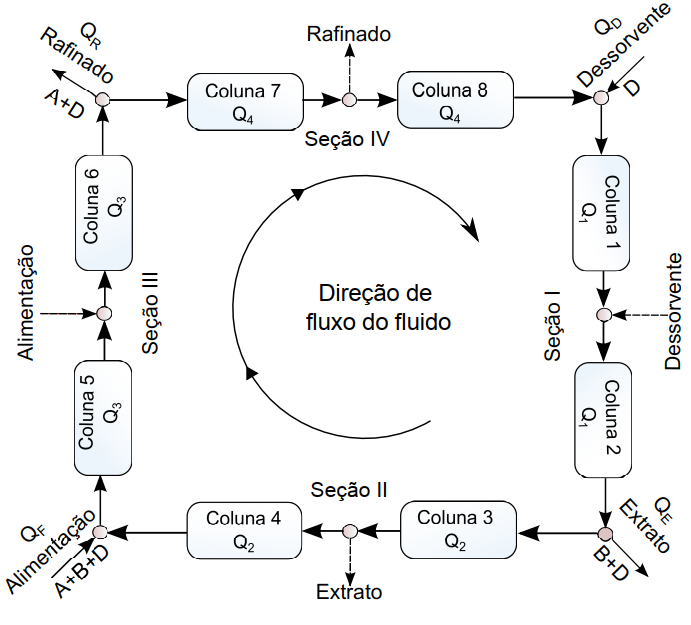
\includegraphics[width=.8\columnwidth]{Arquivos/figura1.png} 
 \caption{Esquema do sistema LMS para oito colunas[Fonte: Oliveira, 2016].} \label{fig-1}
\end{figure}

em que a velocidade de alimentação e a concentração injetada do componente são representadas respectivamente por $v_f$ e $C_{i,f}$.

Porém, a equação de advecção é usada na saída da coluna conforme \cite{haag} representado pela equação,
\begin{equation}
\frac{\partial C_{i,k}}{\partial t} = v_l \frac{\partial C_{i,k}}{\partial x_k}
\end{equation}
 e na fase estacionária a condição de contorno usada é,
 \begin{equation}
 q_{i,k}(t,x_k = L_c) = q_{i,k+1}(t, x_{k+1} = 0)
 \end{equation}

\section{Problema Direto}
A solução do problema direto é essencial para o algoritmo estimar os parâmetros utilizados para os dados experimentais. Por isso é necessário que ela seja fiel em simular os dados experimentais reportados na literatura.

Para solucionar numericamente as Equações Diferenciais Parciais (EDP) com o Método de Linhas (MOL) é aplicada a aproximação utilizando a técnica da diferença centrada de segunda ordem para resolver a equação do termo difusivo, chegando à Eq. 9,
\begin{equation}
\frac{\partial^2 C_{i,k}}{\partial x^2} = D_{ax}(\frac{C_{i,k}^{n,j-1} - 2C_{i,k}^{n,j} + C_{i,k}^{n,j+1}}{2\Delta x})
\end{equation}
Porém, para o termo advectivo utilizados a técnica da diferença centrada de dois pontos, resultando em
\begin{equation}
\frac{\partial C_{i,k}}{\partial x} = - v_l (\frac{C_{i,k}^{n,j+1} - C_{i,k}^{n,j-1}}{2\Delta x})
\end{equation}
Foi utilizado o método de Runge-Kutta de 4 Ordem que é reconhecido pela sua acurácia para solucionar o sistema de EDO.

\subsection{Simulação do problema direto}
Na simulação do modelo matemático utilizado (ver Fig. 2), observa-se boa acurácia com os resultados experimentais na separação de enantiômeros de bi-naftol.
\begin{figure}[H] 
	\centering
	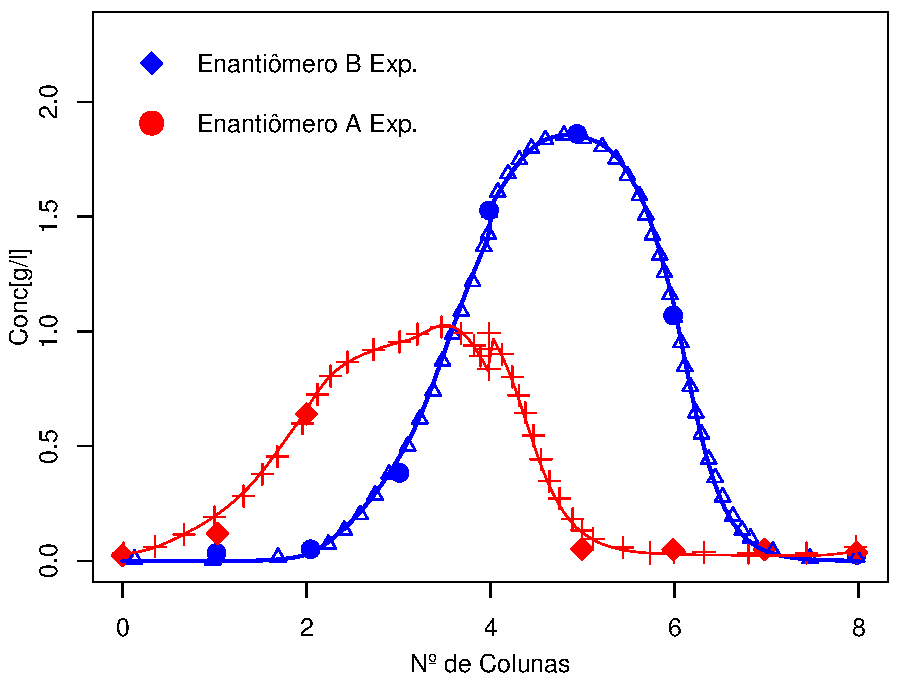
\includegraphics[width=.8\columnwidth]{Arquivos/problema.pdf} 
	\caption{Comparação do modelo matemático com os dados experimentais.} 
\end{figure}

Na Fig. 2 os símbolos \ding{108} e \ding{117} são os valores de concentrações obtidos experimentalmente, enquanto que os $\vartriangle$ e \ding{53} são os resultados analíticos, encontrado na literatura\cite{pais} do modelo matemático usado. Enquanto que as linhas representam os dados encontrados pelo algoritmo.
\section{Problema Inverso}
A solução do problema inverso é uma estimativa dos parâmetros usados para conseguir um conjunto de dados que representa os parâmetros do modelo. Em uma função, descrevemos que desejamos encontrar o valor de $x$ a partir dos valores de $y$, dessa forma, descrita como $y = f(x, \varepsilon_Y)$ , onde $\varepsilon_Y$ é o erro relacionado ao ruído e modelo utilizado. O modelo utilizado, é $f:\mathfrak{R}^n \times \mathfrak{R}^m \Rightarrow \mathfrak{R}^M$ 
, onde $y \in \mathfrak{R}^m$ é quantidade medida e $x \in \mathfrak{R}^n$ é o número de parâmetros a ser encontrado. Os ruídos sintéticos utilizados nesse trabalho foram gerados seguindo a Eq. 11,
\begin{equation}
Y = \widetilde{Y} + \varepsilon_{\widetilde{Y}}, \varepsilon_{\widetilde{Y}} \sim N(0, \sigma_{\widetilde{Y}})
\end{equation}
sabendo que $\widetilde{Y}$ são os dados experimentais reais e $Y$ os dados experimentais com ruído simulado \cite{claudir_emmc}, esses dados experimentais sintéticos são demonstrados na Fig. 3, que mostra no gráfico a linha da função para os parâmetros calculados e os pontos os dados experimentais sintéticos com $\sigma_Y = 0,05$ dando a porcentagem total de ruído de 5\%.
\begin{figure}[H] 
	\centering
	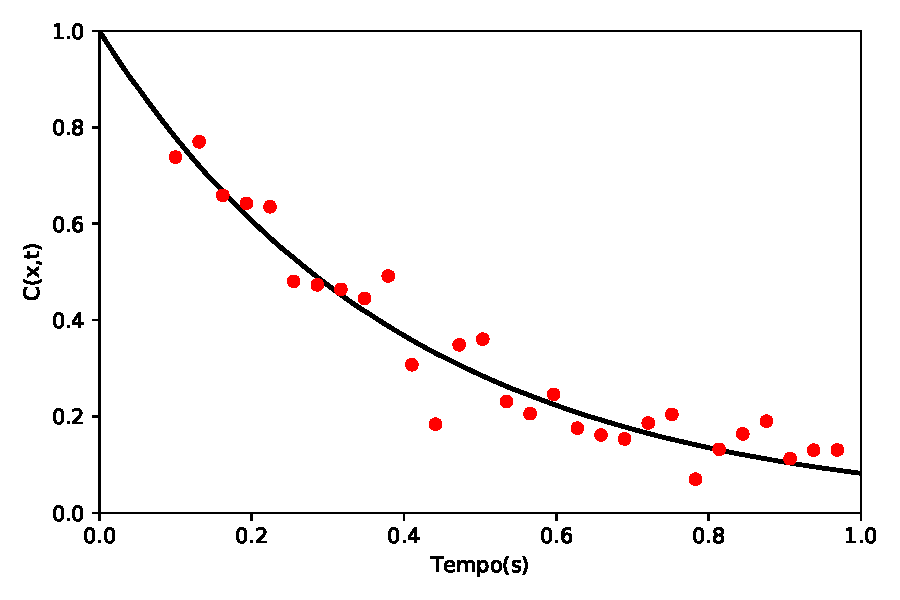
\includegraphics[width=.8\columnwidth]{Arquivos/plot.pdf} 
	\caption{Dados analíticos comparados aos dados experimentais sintéticos.} 
\end{figure}
O problema inverso se baseia na comparação de duas estimativas,  ambas resolvidas pelo algoritmo de Evolução Diferencial que determinará o mínimo da função objetivo por meior da abordagem da Máxima Verossimilhança (MLE), que é quando não existe nenhuma infomação a priori e a Máxima a Posteriori (MAP) que neste caso, supoem-se que existe alguma informação a priori a respeito da solução.

Como critério de escolha dos parâmetros que serão estimados pelas abordagens é necessário analisar a influência dos parâmetros sobre os dados dos perfis de concentração. Por isso é necessário o estudo de sensibilidade desses parâmetros. Neste trabalho utilizou-se as análise já realizadas para os parâmetros de acordo com \cite{claudir_tese}. Os parâmetros ideais para uso em estimativa é necessário que estes sejam linearmente independente \cite{lugon}. Foram escolhidos os parâmetros correspondente ao coeficiente de Henry para a componente A da solução para o sítio 1 e 2 apresentada, respectivamente, nas Fig. 4 e 5. A motivação para escolha desses parâmetros é que este apresentaram alta sensibilidade, o que aumenta as chances de encontrar estimativas precisas, segundo a literatura\cite{vasconcelos}. 
\begin{figure}[H] 
	\centering
	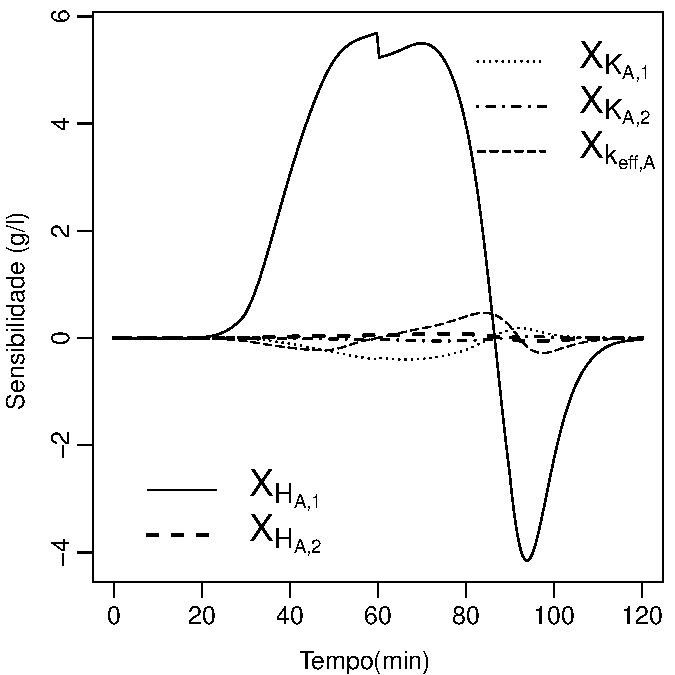
\includegraphics[width=.8\columnwidth]{Arquivos/SensibilidadeCa-all.pdf} 
	\caption{Gráfico de sensibilidade com o parâmetro $H_{A,1}$ [Fonte: Oliveira, 2016]} 
\end{figure}

\begin{figure}[H] 
	\centering
	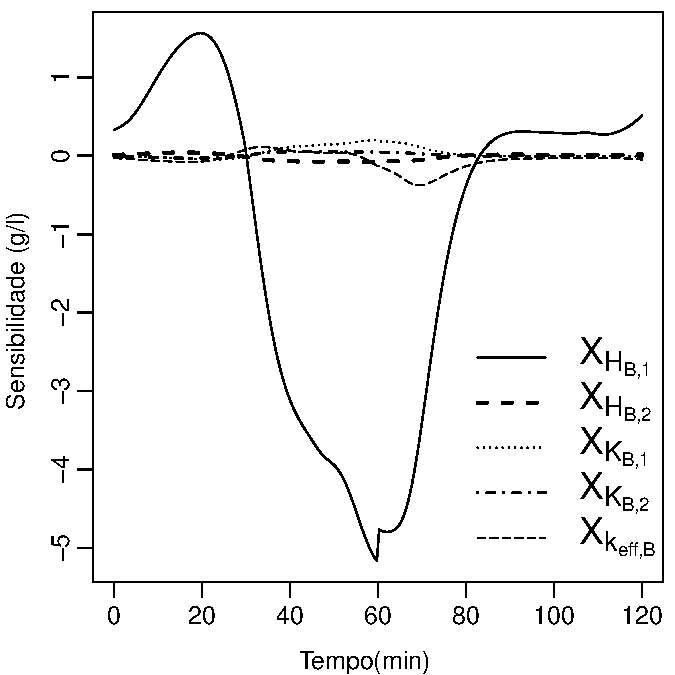
\includegraphics[width=.8\columnwidth]{Arquivos/SensibilidadeCb-all.pdf} 
	\caption{Gráfico de sensibilidade com o parâmetro $H_{A,2}$ [Fonte: Oliveira, 2016]} 
\end{figure}

Essas estimativas permitem determinar uma aproximação dos dados que não podem ser obtidos experimentalmente ou são muito caros computacionamente para serem obtidos.
\section{Máxima Verossimilhança}
A estimativa por Máxima Verossimilhança (Maximum Likelihood Estimation – MLE) funciona através do ajuste de dados estimando os parâmetros através de modelos estatísticos. A função objetivo é a distância do modelo calculado e os dados experimentais. Quando se admite que o modelo é perfeito e as flutuações dos erros experimentais são conhecidas e com distribuição normal, tem-se a função de densidade de probabilidade dos desvios entre o experimento, que deve ser maximizada. Nesse caso, a função é dada por Kaipio \& Somersalo \cite{kapio_book}.
\begin{equation}
\begin{split}
p(Y|Z)= \frac{1}{\sqrt{(2\pi)^{N_d}}}|W|^\frac{1}{2}\times exp(-\frac{1}{2}[Y-C(Z)]^T\\ W^{-1}[T-C(Z)])
\end{split}
\end{equation}
em que $Y$ e $C$ são vetores que correspondem respectivamente, aos dados experimentais e calculados, $Z$ é o vetor de parâmetro, $W$ é a matriz de covariância dos erros experimentais e $N_d$ é a quantidade de dados.

A função da máxima verosimilhança é um problema de otimização que se faz necessária minimizar o funcional de resíduos quadrados entre as quantidades de medidas experimentalmente e os valores calculados pelo modelo. A função objetivo, portanto, é utilizada no procedimento de inversão e é dada pela Eq. \ref{equacaoresiduo} a qual resulta em parâmetros com variância mínima.
\begin{equation}\label{equacaoresiduo}
R(Z) = [Y_i - C_i(Z)]^T [Y_i - C_i (Z)] = \sum_{i=0}^{N_c}[Y_i - C_i(Z)]^2
\end{equation}

\section{Máximo a Posteriori(MAP)}
Essa estimativa se desenvolve da premissa de que existem informações \textit{a priori} dos parâmetros na forma de uma distribuição Gaussiana e que $Y$ e $Z$ são independentes e então é utilizada para a minimização da função objetivo. Do teorema de Bayes tem-se que,
\begin{equation}
p(Z|Y)= \frac{p(Y|Z)q(Z)}{p(Y)}
\end{equation}
onde $q(Z)$ é a probabilidade \textit{a priori}, ou seja, é a probabilidade da amostra para o parâmetro $Z$, podendo ser estimado pela Eq. 15,
\begin{equation}
q(Z)=2\pi^{\frac{-N_{un}}{2}}|V^{-\frac{1}{2}}| \times exp(-\frac{1}{2}[Z-\mu_{pr}]^T V^{-1}[Z-\mu_{pr}])
\end{equation} 
sabendo que $\mu_{pr}$ é a informação a priori e $V$ é a matriz de covariância. Aplicando a função de logaritmo natural ao teorema geral de Bayes, obtem-se a Eq. 16,
\begin{equation}
ln(p(Z|Y))=ln(q(Z))+ln(p(Y|Z))-ln(p(Y))
\end{equation}
que substituindo, na Eq. 16, as Eq. 15 e 12, e resolvendo e manipulando as equações é obtido a Eq. 17,
\begin{equation}
\begin{split}
ln(p(Z|Y)) = -\frac{1}{2}[(N_{un}+N_d)ln(2\pi)+ln|V^{-1}|+\\
ln|W^{-1}|+F_{map}(Z)]
\end{split}
\end{equation} 
tomando que a função $F{map}(Z)$, é
\vspace{10pt}
\begin{equation}
\begin{split}
F_{map}(Z)=([Y-C(Z)]^TW^{-1}[Y-C(Z)]+\\
[Z- \mu_{pr}]^T V^{-1}[Z-\mu_{pr}])
\end{split}
\end{equation}
Supondo que vetor $Z$ maximiza $ln(p(Z|Y))$ é igual a $max(p(Z|Y))$, então implica na Eq. 19,
\begin{equation}
_\mathbf{Z}^{max} p(Z|Y) \Leftrightarrow _\mathbf{Z}^{max} [ln(p(Z|Y))] \Leftrightarrow _\mathbf{Z}^{min} [F_{map}(Z)]
\end{equation}
onde, $Z$ corresponde ao vetor das amostras aleatórias com média $\mu$ e matriz de covariância conhecida $V$ que introduzem informação \textit{a priori} a respeito do vetor $Z$. A minimização de $F_{map}$ produz estimativas de $Z$ que maximizam a distribuição \textit{a posteriori} $p(Z|Y)$.

\section{Evolução Diferencial (DE)}
O algoritmo de evolução diferencial é um algoritmo que tem como finalidade a otimização de uma função. É um método estocástico que se inspira na teoria da evolução e seleção natural \cite{Storn}.

É descrito como um algoritmo que tem como função a manipulação de uma população de indivíduos $N_{pop}$ que representam as soluções da otimização \cite{leppaus}. Ao passar das gerações esses candidatos passam por processos nomeados de \textit{mutação} e \textit{cruzamento}, que tem o intuito de criar soluções melhores para que possam passar pela \textit{seleção} para poder iniciar uma nova geração.

Inicialmente, é gerado uma população de números $N_{pop}$ a partir da Equação 20,
\begin{equation}
\begin{split}
X_{i,j}=X_{j,lower}+r_{ij} (X_{j,upper}-X_{j,lower}),\\
i = 1,...,N_{pop}, j =1, ..., N_p
\end{split}
\end{equation}
onde $X_{j,lower}$ e $X_{j,upper}$ são intervalo de busca mínimo e máximo, respectivamente, $N_p$ é a quantidade de parâmetros e $r_{ij}$ é o número real aleatório gerado dentro do intervalo de 0 a 1.

Após a geração da população entra em fase a parte de \textit{mutação} dos indivíduos. Todos os indivíduos da população são modificados através da Eq. 21, onde é retirada a diferença entre dois indivíduos  diferentes $X_{l_2}$, $X_{l_3}$, escolhido aleatoriamente e feito produto com uma taxa de perturbação $F$, gerado aleatoriamente entre 0 e 2, e então somado ao vetor de referência $X_{l_1}$, para gerar um terceiro indivíduo.
\begin{equation}
X_{l,new}=X_{l_1} + F(X_{l_2} - X_{l_3})
\end{equation}
Sendo que esse novo indivíduo deve passar pela etapa de cruzamento, que é o processo de decisão para adicionar o novo indivíduo a população, se não, é mantido  indivíduo anterior $X_{l_1}$m representado pela Equação 22, que $C_r$ é a probabilidade de mutação, e $r_1$ é o número real aleatório do intervalo de 0 a 1.
\begin{equation}
X_l= \left\{\begin{matrix}
X_{l,new},\hspace{7pt} \mathrm{se}\hspace{7pt} r_1 < C_r \hspace{7pt}\mathrm{ou} \hspace{7pt} j = j_{rand}\\
 X_{l_1},\hspace{7pt} \mathrm{caso} \hspace{7pt}\mathrm{contrário}

\end{matrix}\right.
\end{equation}

\section{Resultados e Discussões}

Sabendo a influência dos parâmetros no perfil de concentração, é possível estimar a partir dos métodos de \textit{máxima verosimilhança} e \textit{máximo a posteriori}. Para este trabalho foram utilizados 13 execuções visando obter um conjunto de soluções a partir do método DE. A probabilidade de mutação foi definido com $C_r = 0,9$ e o número da população $N_{pop} = 30$ como critério de parada sendo o número de gerações igual a 80. Também foi definindo o intervalo de busca de acordo com os valores de referência para cada parâmetro, apresentado na Tab. 1.
\begin{table}[!h]
	\centering
	\caption{Intervalo de busca para o modelo estocástico.} \label{tabela-1}
	{\small
		\begin{tabular}{ccccc}			
			\hline
			\hline
			\thead{Parâmetros} & \thead{Valor de Ref.} & \thead{$L_{min}; L_{max}$} \\
			\hline
			\hline
			$H_{A,1}$ & 2,69 & $[1;3]$\\
			$H_{A,2}$ & 0,1 & $[0;0,5]$\\
			\hline
			\hline
	\end{tabular}}
\end{table}
No término das execuções foram calculados a média o desvio padrão e o coeficiente de variação dos parâmetros da isoterma para as estimativas do MLE e MAP conforme apresentado na Tab. 2.
\begin{table}[!h]
	\centering
	\caption{Resultado da estimativa com valor de referência} \label{tabela-2}
	{\small
		\begin{tabular}{ccccc}			
			\hline
			\hline
			\thead{} &  \thead{Parâmetros} & \thead{$H_{A,1}$} & \thead{$H_{A,2}$}\\
			\hline
			\hline
			 & Média($\mu$) & 2,6782 & 0,1636 \\
			 MLE & Desvio($\sigma$) & 0,0098 & 0,0364\\
			 & ($\sigma / \mu) \times 100$ & 0,3641 & 22,2310 \\
			 \hline
			 & Média($\mu$) & 2,6887 & 0,1184\\
			 MAP & Desvio($\sigma$) & 0,0088 & 0,0309\\
			 & ($\sigma / \mu) \times 100$ & 0,3285 & 26,0985 \\
			\hline
			Valor de Ref. &  & 2,69 & 0,1 \\
			\hline
			\hline
	\end{tabular}}
\end{table}

O desvio padrão relativo ou coeficiente de variação é dado por $\mu/\sigma \times 100$ que representa um número adimensional que serve para analizar a variabilidade de dados e é utilizada quando se quer fazer comparações da variação de conjuntos de soluções que são diferentes na média. Para os parâmetros em estudo mostra-se que quanto menor for o seu valor, mais homogêneos são os conjuntos obtidos pelas estratégias.
 
\section{Conclusão}
O intuito deste trabalho foi analisar o modelo estocástico de Evolução Diferencial na minimização da função objetivo. Considerando os resultados apresentados, verifica-se que o método se mostra promissor considerando os resultados de outros modelos citados na literatura, como por Oliveira\cite{claudir_tese}. Verifica-se que abordagem \textit{a posteriori} não se mostrou eficiente para esta aplicação. Isso pode ser justificado pelo os ajustes dos desvios padrão utilizados, correspondente a informação a priori. Pode-se considerar, no entanto, que o método foi eficaz em aplicações reais. Como trabalho futuro, o método será aplicado para a determinação dos demais parâmetros existente no modelo usado, conforme identificados nos gráficos da análise de sensibilidade.




%\section{Agradecimentos}
%
%\appendix
%\section{Apêndices}
%Use a seção apêndice quando necessário.
%\subsection{Demonstracões}
%\subsection{Algoritmos}

%\insertbibliography{Referencias.bib}
\bibliographystyle{IEEEtran}
\bibliography{IEEEabrv,Referencias}

\end{document}
